\documentclass{article}
\usepackage[paperwidth=210mm,paperheight=297mm, top = 30mm, bottom = 30mm]{geometry}
%\usepackage[hangul]{kotex}
\usepackage{kotex}
\usepackage[utf8]{inputenc}
\usepackage{enumitem}
\usepackage{indentfirst}
\usepackage{graphicx, subcaption, tikz}
\usepackage{amsmath, amssymb, amsthm, amsfonts, bm}

\title{2020 Spring MAS365 Numerical Analysis HW6}
\author{20160650 채지석}
\date{\today}

\setlist{  
  listparindent=\parindent,
  %parsep=0pt,
}

\newtheorem{prob}{Problem}

\newcommand{\set}[1]{\left\{ {#1} \right\}}
\newcommand{\vecx}{\boldsymbol{x}}
\newcommand{\mat}[1]{\boldsymbol{#1}}
\newcommand{\mata}{\boldsymbol{A}}
\newcommand{\matb}{\boldsymbol{B}}
\newcommand{\rr}{\mathbb{R}}
\newcommand{\nn}{\mathbb{N}}
\newcommand{\zz}{\mathbb{Z}}
\newcommand{\cc}{\mathbb{C}}
\newcommand{\qq}{\mathbb{Q}}
\newcommand{\norm}[1]{\left\lVert#1\right\rVert}
\newcommand{\card}[1]{\left\lvert#1\right\rvert}
\newcommand{\posdef}{\succ\mat{0}}
\newcommand{\psd}{\succeq\mat{0}}
\newcommand{\trace}{\text{trace}}
\newcommand{\comment}[1]{}
\newcommand{\problem}{\begin{prob}\end{prob}}
                    

\begin{document}

\section*{Computer Assignment}
The program which does the required is submitted via KLMS along with this document. Given the two endpoints of the interval \texttt{a} and \texttt{b}, the step size \texttt{h}, and a function \texttt{f}, the program computes the interpolating polynomial using the divided difference scheme. The computed interpolating polynomials are printed out, as the following figure. 
\begin{center}
    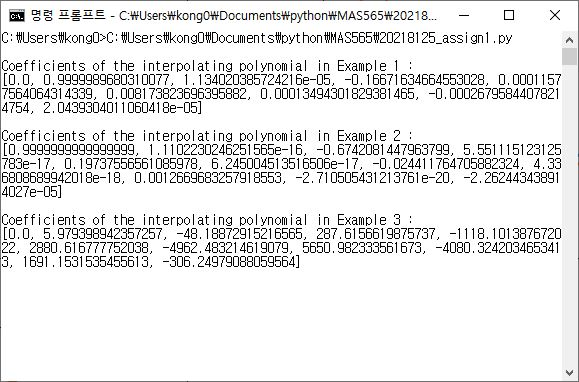
\includegraphics[width=0.8\linewidth]{console.JPG}
\end{center}
The results are the list of coefficients of the resulting polynomial, from the lowest degree term to the highest. For example the first result indicates that the interpolating polynomial is \[
p(x) = 0.0 + 1.000 x + 1.134\times 10^{-5} x^2 + \cdots + 2.044\times 10^{-5} x^8. 
\] The original function $f$ and the interpolating polynomial $p$ plotted together, for each example, is shown as in the following figure. 
\begin{center}
    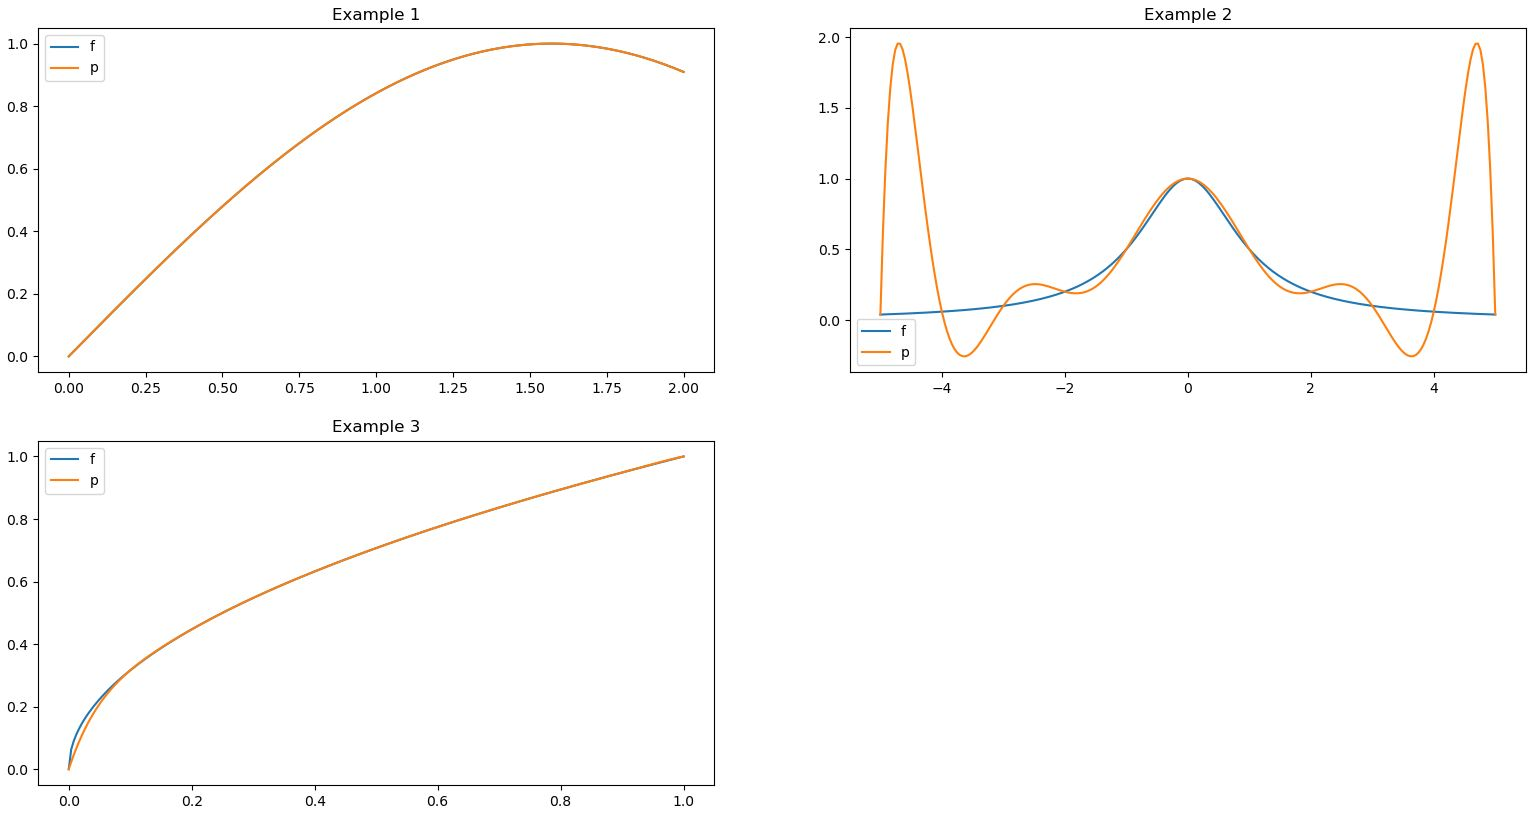
\includegraphics[width=\linewidth]{3313.JPG}
\end{center}
The first function $f(x) =\sin x$ looks well interpolated by the interpolating polynomial. Such a behavior is actually exactly as expected, because we have $\norm{f^{(n)}(x)}_\infty \leq 1$ for any positive integer $n$, exactly the case discussed in Problem 2.4. \par 
The second function, the Runge function $f(x) = \dfrac{1}{1+x^2}$, is badly interpolated, especially on the region near the end points of the given interval. It is indeed an example of a function where increasing the number of nodes does not increase the quality of the interpolation. \par 
The third function $f(x) = \sqrt{x}$ is also not so well interpolated near $x=0$. Indeed $f$ has a vertical asymptote at $x=0$, which is a trait a polynomial cannot have. As a result the error is even visible with our bare eyes.   
\end{document}